\chapter{Introduction} \label{chap:introduction}

%The aim of this project is to investigate the possibilities of a novel concept of airfoil twist morphing.

%Describe a little bit what is morphing...
Aircraft morphing is a very broad term that can be understood as the modification of the geometry of the aerodynamic surfaces to enhance the performance through the adaptation to the current flight condition. The interest in morphing of aerodynamic surfaces has accompany aerospace history since the beginning. In 1903, the Wright Brothers successfully completed the first heavier-than-air flight when they designed and build a powered aircraft that achieved a controlled and sustained flight. Their design incorporated a mechanism that provided lateral control by manually changing the twist of the wing. Since then, the necessity of enhanced performance and higher airspeed brought the requirement of stiffer wing structures that would provide increased load carrying capabilities and improved protection against aeroelastic instabilities, among other benefits. As a result, research focused on improving the design of structures that did not exploit the elastic capabilities of the materials used.

%Why to used them?
On conventional transonic airliners, the need to modify the airflow around the airfoil at different flight conditions is achieved through discrete hinged mechanics such as flaps and ailerons. These mechanisms fulfill its mission in a limited range around the design point while, outside this range, they have a negative influence in the aerodynamics. The necessary discontinuities that these elements produce on the surface advance the boundary layer transition point from laminar to turbulent regime and therefore increase the wing aerodynamic parasite drag. 

%Gust
Being able to modify the airflow without discontinuities on the surface would come along with notable reductions in drag and consequently in fuel consumption. Furthermore, these benefits could be applied to diverse flight conditions or flight path alteration requirements. For example, the modification of the wing swept angle as a common practice to obtain an aircraft able to efficiently fly at a wide range of Mach numbers. Another application of wing morphing is the counteracting of the excessive aerodynamic load originated after gust encountering. This is a flight condition under which aircraft experience critical loads that mark the design point for the airframe due to its structural integrity threat. In such a event, an aircraft is flying in turbulent air and a component of the air velocity, normal to the flight path, changes the effective angle of incidence of the aerodynamic surfaces increasing its aerodynamic load. In Figure \ref{fig:gust}, the case of an aircraft encountering a vertical gust is shown. Several mechanisms, which usually add structural mass, have been developed to withstand this rare but critical scenarios. Such solutions require a rapid modification of the lift distribution that mitigate the increment in aerodynamic load. In some modern transonic aircraft, after a gust encountering, the ailerons of both wings are deflected in such a way that they reduce the local airfoil chamber, reducing as well the lift generated at the wing tip.

\begin{figure}[!htpb]
  \centering
  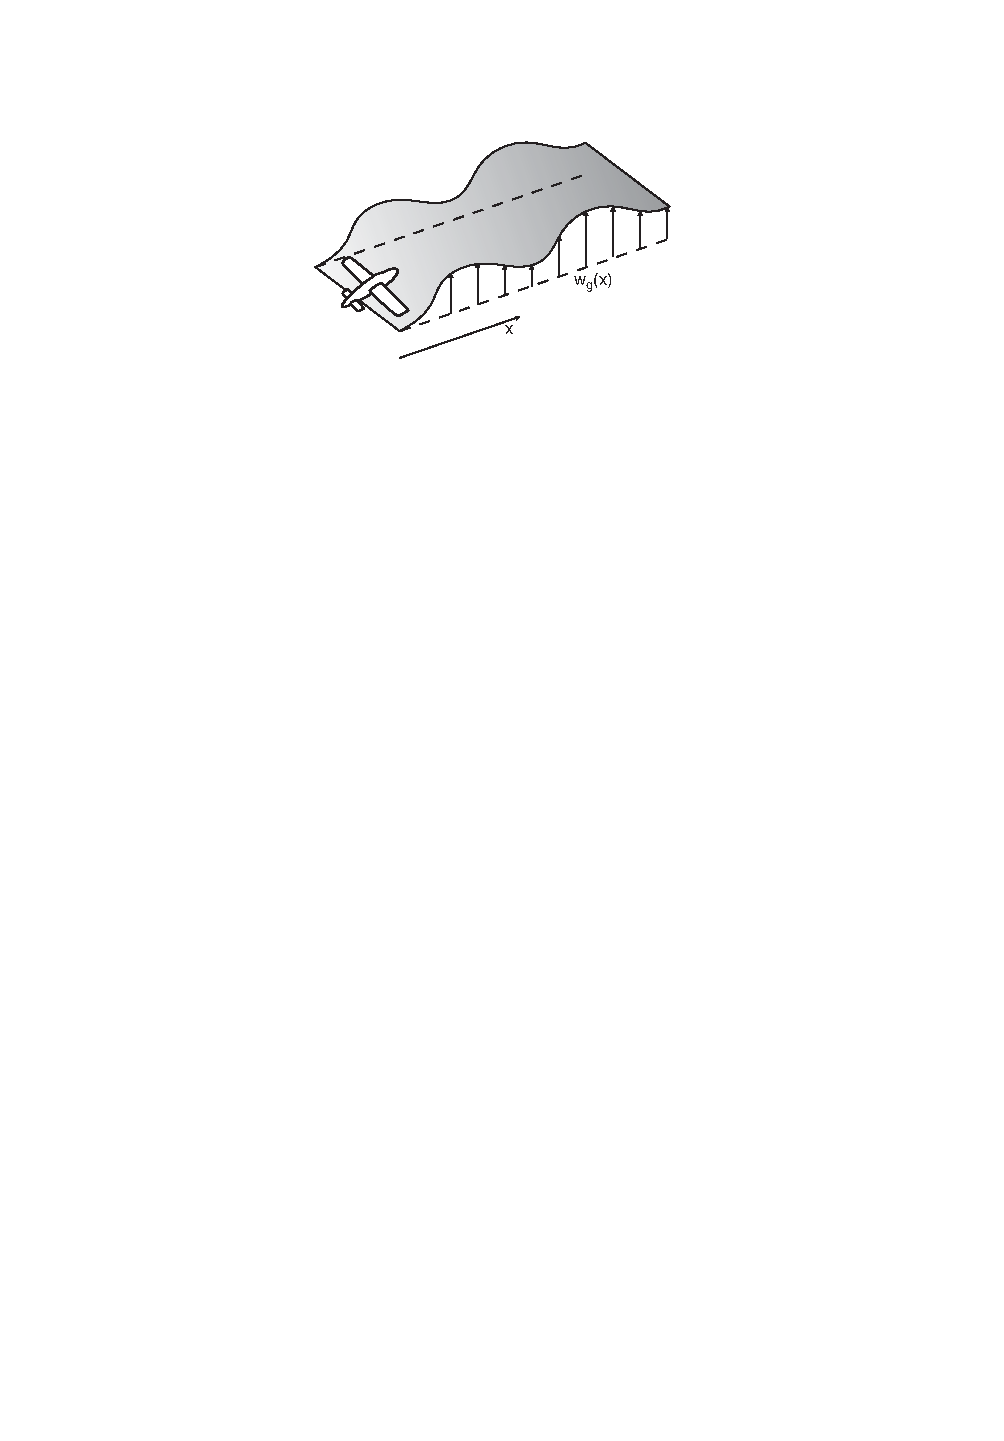
\includegraphics[width=0.7 \textwidth]{state-of-the-art/gust}
  \caption[Aircraft encountering a vertical gust]{Aircraft encountering a vertical gust. \cite{JECooper2007}}\label{fig:gust}
\end{figure}

For the particular objective of load alleviation, a wing morphing design needs to show compliance with a time bounded response. Having achieved this requirement, the advantages of using such an approach include weight reduction and/or the no alteration of the aerodynamic surfaces continuity with hinges, which provide reduced operation costs and aerodynamic performance enhancement, respectively.

The present work is a proposal of a novel wing morphing technology. Through wing twist modifications, it is possible to reduce the angle of attack and limit the aerodynamic load on the wings. The presented concept consists on a mechanism able to modify the torsional stiffness of the wing-box through the inclusion of a variable-stiffness spar. The modification of the effective shear modulus in this element provokes the wing-box shear center shifting and the consequent modification in wing-box torsional stiffness. 

The activation of the adaptive spar is an event fully passive and its based on the appearance of elastic controlled instabilities in the structure of the spar. This element is constituted of a lattice of chiral structures, which consists on a network of interconnected nodes and ligaments. Under certain load, some of the ligaments in the lattice start to buckle eventually causing the collapse of the structure due to the sudden reduction of the shear stiffness in the spar. This event induces a sudden variation in the wing-box twist as its torsional stiffness is altered.

The objectives for the work presented in this thesis include the evaluation of the buckling mechanism as a valid trigger for the variable-stiffness spar adaptation and consequent variation of the wing-box twist. In other words, to show how local buckling can affect the global morphing behavior. Also, the elastic instability or buckling that undergoes in the spar is aimed to be characterized by qualitative means. Finally, the possibility of tailoring the deformation response by varying structure parameters is intended to be evaluated. 

This thesis is organized as follows: succeeding this introduction, the state-of-the-art of the technologies related to the one proposed in this work are presented. Then, the wing-box model, developed to investigate the proposed morphing mechanism, is described in the third chapter, following a characterization of its mechanical properties in the subsequent chapter. The fifth chapter shows the results obtained from the simulations performed on the computational model of the wing-box. The conclusion and outlook complete this thesis.